\documentclass[a4paper,12pt]{report}
\usepackage[T1]{fontenc}
\usepackage[utf8]{inputenc}
\usepackage[francais]{babel}
\usepackage[usenames,dvipsnames,svgnames,table]{xcolor}
\usepackage[colorlinks,linkcolor={blue!30!black},citecolor={blue!50!black},urlcolor={blue!80!black}]{hyperref}
\usepackage{amsmath,array,graphicx,caption,lmodern,subcaption,tikz,url,xspace,wrapfig}
\usepackage{textcomp,rotating,epic,eepic,pdfpages}
\usepackage[top=2cm,left=2.5cm,right=2.5cm,bottom=2cm]{geometry} % Géométrie de la page, modifier selon le besoin
\usepackage[babel=true,kerning=true]{microtype}

\addto{\captionsfrench}{\renewcommand{\abstractname}{Introduction}}
\pdfsuppresswarningpagegroup=1
\date{}
\title{Rapport de Stage d'Application}
\author{Félix Piédallu}


\begin{document}
\nocite{*}
\pagenumbering{gobble}  % Pas de numérotation
\begin{titlepage}
    \vspace*{-10px}
    
\includegraphics[height=80px]{Images/logo_phelma.pdf}
    \vspace*{-80px}
\begin{flushright}
    \vspace*{-10px}
    
\includegraphics[height=80px]{Images/Logo_Neel.pdf}
\end{flushright}

\vspace*{1.5cm}
\begin{center}
\rule{\linewidth}{0.5mm}\\[0.4cm]
{\huge{\bfseries Rapport de Projet de Fin d'Études}\\[0.4cm]
Développement d'une nanopince optique fibrée plasmonique originale\\[0.4cm]}
\rule{\linewidth}{0.5mm}\\[0.5cm]

\LARGE{\textsc{Félix Piédallu}}\\[0.7cm]
\large{\textsc{Filière PNS 2015-2016}}\\[2cm]

\Large{Au sein de l'équipe Nano-Optique et Forces}\\[1cm]

\Large{Sous la direction de Jochen \textsc{Fick}}\\[2cm]

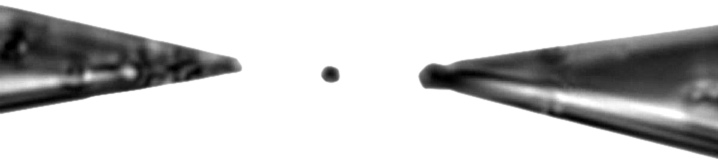
\includegraphics[width=\textwidth]{Images/Illustration.png}\\[1cm]


\end{center}
\end{titlepage}

\tableofcontents        % Table des matières avec liens, générée automatiquement.
\newpage
\pagenumbering{arabic}  % Numérotation de retour !


% Remerciements
%\input{0.Remerciements}

\chapter*{Nano-Optique et Forces}
L'équipe NOF fait partie de l'institut Néel, blablabla.
% , le laboratoire de l'ENS Ulm spécialisé dans la physique de la matière condensée et la physique mésoscopique.

% Elle regroupe autour de Takis Kontos et Audrey Cottet plusieurs doctorants : Matthieu Baillergeau, Matthieu Desjardins, Matthieu Dartiailh et Laure Bruhat, avec qui j'ai essentiellement travaillé durant mon stage.\newline
%
% L'équipe se concentre sur l'utilisation des nanotubes de carbone, en tant que double puits quantique ou qu'atome macroscopique (atome artificiel).
%
% Le nanotube de carbone est placé dans une cavité résonnante dont on fait varier les paramètres, et donc la fréquence de résonnance. Les sujets de recherche sont donc essentiellement concertés autour de la spintronique et du transport quantique dans de tels milieux.
%
% L'équipe met donc en place le modèle théorique d'une part, et s'occupe de la fabrication des échantillons et de la mise en place de l'expérience.\newline
%
% Le laboratoire est équipé d'un cryostat à Hélium3 (Oxford Heliox VL), d'un cryostat à dilution (Kelvinox Oxford MX250) et d'un cryostat à dilution sèche (Cryoconcept Cryofree), sur lequel j'ai travaillé dans le cadre de mon stage.





\chapter*{Introduction} % Contexte du stage
%\input{0.Introduction}

\chapter{L'expérience}
%\input{1.Experience}

\chapter{Le cryostat à dilution}
%\input{2.Cryostat}

\chapter{Le câblage DC et RF}
%\input{3.Cablage}

\chapter*{Bilan}
\addcontentsline{toc}{chapter}{Bilan}




\bibliographystyle{unsrt}
\bibliography{bibliographie}
\listoffigures
\newpage
\appendix
\phantomsection
\addcontentsline{toc}{part}{Annexes}

\vspace*{8cm}
\begin{center}
\rule{\linewidth}{0.5mm}\\[0.7cm]
{\huge{\bfseries Annexes}}\\[0.4cm]
\rule{\linewidth}{0.5mm}\\[0.5cm]


\end{center}
%\newpage
%\phantomsection
%\addcontentsline{toc}{chapter}{Guide de câblage du cryostat}
%\includepdf[pages={-}]{../guide.pdf}

\newpage
%\input{9.Abstract}

\end{document}
